\subsection{Wave equation with bound conditions}
\paragraph{Half-infinite string}
Suppose string is fixed in one of its ends, at $x=0$: $u(0,t) = 0$. This is called Dirichlet boundary condition. We want to solve the PDE for $x>0$.

\subparagraph{Property of wave equation}
If $u(x,t)$ is solution, then $u(-x,t)$ is also solution:
$$u(x,t) = F(x+ct) + G(x-ct)$$
$$u(-x,t) = F(-x+ct)+G(-x-ct) = \bar{F}(x+ct) + \bar{G}(x-ct)$$
Where $\bar{F}(s) = G(-s)$ and $\bar{G}(s) = F(-s)$.

Lets extend $f$ and $g$ on the whole plane in odd way:
$$\bar{f}(x) = \begin{cases}
f(x) & x>0\\
-f(x) & x<0
\end{cases}$$
and same for $g$. 

Note that initial conditions have to be consistent, i.e., $f(0)=0$, $g(0)=0$, else the solution is discontinuous in 0.
Lets use D'Lambert solution:
$$\bar{u}(x,t) = \frac{\bar{f}(x+ct) + \bar{f}(x-ct)}{2} + \frac{1}{2c} \int_{x-ct}^{x+ct} \bar{g}(s) \dd{s}$$
Then the solution of half-infinite string is
$$u(x,t) = \begin{cases}
\frac{f(x+ct) + f(x-ct)}{2} + \frac{1}{2c} \int_{x-ct}^{x+ct} g(s) \dd{s}& x>ct\\
\frac{f(x+ct) - f(ct-x)}{2} + \frac{1}{2c} \int_{ct-x}^{x+ct} g(s) \dd{s}& x<ct\\
\end{cases}$$ 
\paragraph{Neumann boundary condition}
In this case, instead of giving boundary condition on $u$, we give boundary condition of $u_x$: $u_x(0,t) = 0$. Physical meaning is that there is no force in this point. In this case we will extend function in even way (derivative of even function in 0 is 0). Then we get$$u(x,t) = \begin{cases}
\frac{f(x+ct) + f(x-ct)}{2} + \frac{1}{2c} \int_{x-ct}^{x+ct} g(s) \dd{s}& x>ct\\
\frac{f(x+ct) + f(ct-x)}{2} + \frac{1}{2c} \int_{0}^{ct-x} g(s) \dd{s} + \frac{1}{2c} \int_{ct-x}^{x+ct} g(s) \dd{s}& x<ct\\
\end{cases}$$ 
\paragraph{Uniquness}
Suppose we have two solutions, by subtracting them, we get
$$\begin{cases}
u_{tt} -c^2u_{xx} = 0\\u(x,0) = u_x(x,0) = 0\\ u(0,t) = 0
\end{cases}$$
We acquire $u(x,t)=0$. Since $u(x,t)$ is of form $F(x+ct)+G(x-ct)$, we get that two solutions are identical.
\paragraph{Wave equation with finite string}
Suppose we have string from $a$ to $b$:
$$\begin{cases}
u_{tt} - c^2u_{xx} = 0 & a\leq x \leq b \\
u(x,0) = f(x) \\
u_t(a,t) = h(t)\\
u_t(b,t)b= q(t)\\
\end{cases}$$
Here the consistency conditions are
$$\begin{cases}
h(0) = f(a) & q(0) = f(b)\\
h'(0) = g(a) & q'(0) = g(b)
\end{cases}$$
Here we could have conditions derivatives instead of values as well.
\paragraph{Parallelogram identity}

\begin{center}
	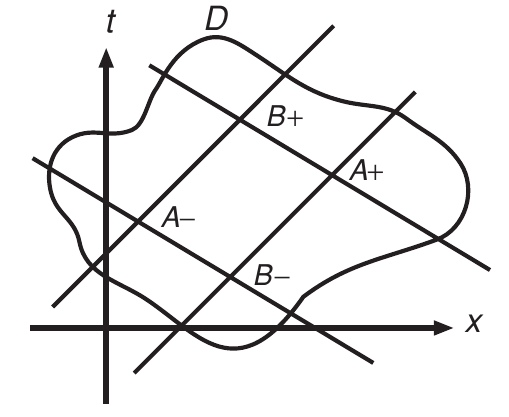
\includegraphics[width=0.4\linewidth]{./lect4/pic1.png}
\end{center}
$u\in \mathcal{C}^2$ is the solution of wave equation iff for any parallelogram with sides parallel to characteristic lines with vertices $A_-$, $A_+$, $B_-$, $B_+$ 
$$u(A_-)+u(A_+) = u(B_-) + u(B_+)$$
\subparagraph{Proof}
One direction is simple, since value of solution is constant along characteristic curves.

For second direction lets switch to canonical coordinates
$$\begin{cases}
\xi = x+ct\\
\eta = x-ct
\end{cases}$$
So
$$w(\xi, \eta) = u\qty(\frac{\xi+\eta}{2} ,\frac{\xi-\eta}{2})$$
$w$ is solution of wave equation iff $w_{\xi \eta} = 0$. 

Note that parallelogram turned into rectangular in new coordinates, i.e.,
$$w(\xi_0, \eta_1) + w(\xi_1, \eta_0) = w(\xi_1, \eta_1) + w(xi_0, \eta_0)$$
Dividing by $(\xi_1-\xi_0)(\eta_1-\eta_0)$:
$$\frac{w(\xi_0, \eta_1) + w(\xi_1, \eta_0) }{(\xi_1-\xi_0)(\eta_1-\eta_0)} - \frac{w(\xi_1, \eta_1) + w(xi_0, \eta_0)}{(\xi_1-\xi_0)(\eta_1-\eta_0)} = 0$$
Taking limit:
$$\lim_{\xi_1\to \xi_0} \lim_{\eta_1\to \eta_0} \frac{w(\xi_0, \eta_1) + w(\xi_1, \eta_0) - w(\xi_1, \eta_1) -  w(xi_0, \eta_0)}{(\xi_1-\xi_0)(\eta_1-\eta_0)} = w_{\xi\eta} = 0$$


In this way we can solve wave equation on finite range:
\begin{center}
	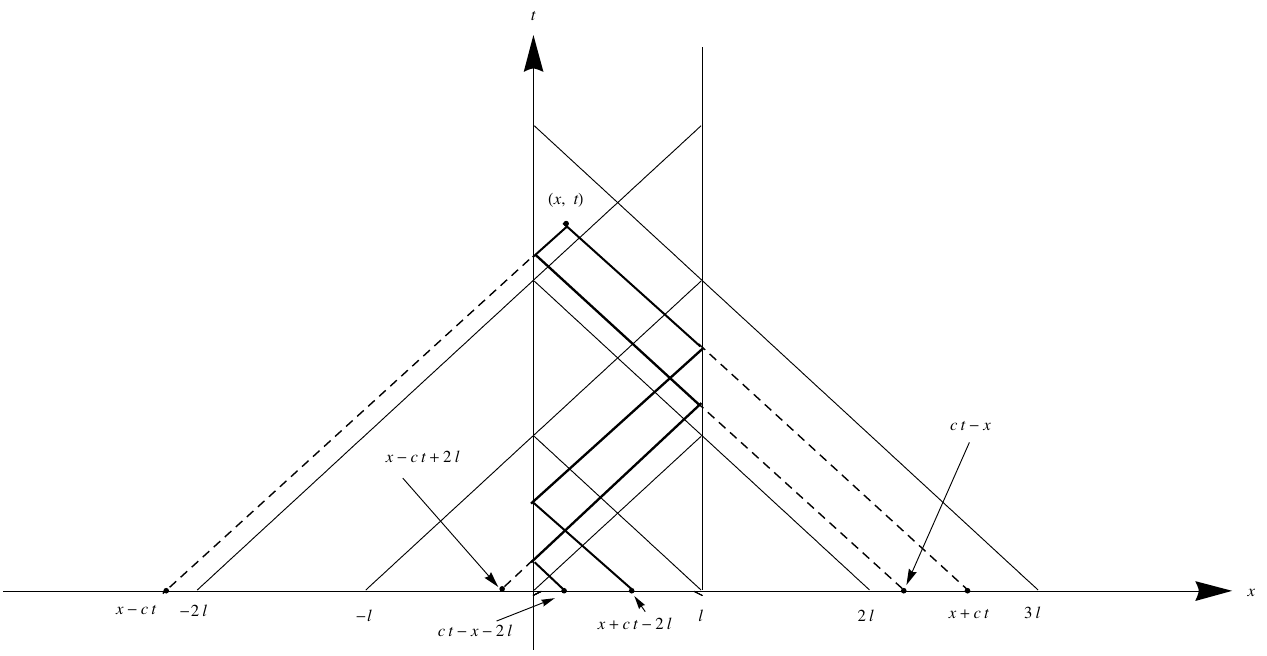
\includegraphics[width=\linewidth]{./lect4/pic2.png}
\end{center}
Using this method we can get solution for homogeneous wave equation for finite string.
\paragraph{Non-homogeneous wave equation}
$$u_{tt} -c^2u_{xx} = \varphi(x,t)$$
In this case parallelogram identity doesn't work. 

Lets extend $\varphi$ to the half plane $x>0$ to some function $\tilde{\varphi} \in \mathcal{C}^1$.


Lets solve non-homogeneous equation with 0  initial conditions:
 $w= \frac{1}{2c}\int\limits_{\triangle} \tilde{\varphi}$.


 with D'Lambert formula. 
 Lets solve homogeneous equation in the interval:
 $$\begin{cases}
 v(a,t) = h(t) + w(a,t)\\
 v(b,t) = q(t)+ w(b,t)\\
 v(x,0) = f(x)\\
 v_t(x,0) = g(x)
 \end{cases}$$
 
 Then the solution is
 $$u(x,t)= w(x,t)+v(x,t)$$
Checking the solution:
$$u_{tt} - c^2u_{xx}=  w_{tt} - c^2w_{xx} + v_{tt} - c^2v_{xx} = \tilde{\varphi}(x,t)  $$
which is $\varphi(x,t)$ in our interval.
\paragraph{Energy method}
Define
$$E(t) = \int_a^b \qty[ u_t^2(x,t) + c^2u_x^2(x,t)] \dd{x}$$ 
If $u\in \mathcal{C}^2$ we can differentiate it:
$$\dv{E}{t} = \int_a^b \qty[2u_tu_{tt} + 2c^2u_xu_{xt}] \dd{x} = 2c^2\int_a^b \qty[u_t u_{xx} + u_xu_{xt}]\dd{x} = 2c^2 \int_a^b (u_xu_t)_x \dd{x} = 2c^2 \qty[u_x(b,t)u_t(b,t) - u_x(a,t) u_t(a,t)]$$
If any combination of Dirichlet and Neumann conditions is fulfilled, the integral is $0$, i.e., energy is conserved. Thus
$$E(t) = E(0) = \int_a^b g^2(x) + c^2\qty(f'(x))^2 \dd{x}$$

From that we can conclude the solution is unique. As usual, suppose there are two solutions, $u$ and $v$. Subtracting we get a solution for homogeneous equation with homogeneous initial conditions $w=u-v$. Then $E_w(t) = E_w(0)=0$, thus $w_x=w_t=0$ and $w(x,t)=0$.

Also, from energy difference, we can conclude the solutions are stable.
\subsection{Variable separation}
Lets guess solution of form
$$U(x,t) = A(x)B(t)$$
Substituting into wave equation:
$$u_{tt} - c^2u_{xx} = A(x)B''(t) - c^2A''(x) B(t) = 0$$
Dividing by $A(x)B(t)$ (assume they are not zero):
$$\frac{B''(t)}{B(t)} = c^2\frac{A''(x)}{A(x)} = \mu$$
That means
$$\begin{cases}
A'' = \frac{\mu}{c^2}A = -\lambda A \\
B'' = \mu B
\end{cases}$$

Back to initial conditions $u(0,t)=u(1,t)=0$, that means $A(0) =A(1) = 0$. The question is when
$$A''+\lambda A = 0 $$
If $\lambda< 0$, the solution is
$$A = \alpha e^{-\sqrt{-\lambda}x} + \beta e^{\sqrt{\lambda}x}$$
Substituting initial conditions we get
$$\begin{cases}
\alpha+\beta=0\\
\alpha e^{-\sqrt{-\lambda}} + \beta e^{\sqrt{-\lambda}} = 0
\end{cases}$$
Since $\lambda\neq 0$, we conclude $\alpha=\beta=0$ which is trivial solution.
If $\lambda=0$ we get $A=\alpha x+\beta$, which is also trivially $A=0$.
If $\lambda>0$,
$$A = \alpha \sin(\sqrt{\lambda}x)+ \beta\cos(\sqrt{\lambda}x)$$
Since $A(0) = 0$, $\beta=0$. Since $A(1) = 0$, $\sqrt{\lambda} = k\pi$ for some $k \in \mathbb{N}$, i.e., $\lambda_k = k^2\pi^2$. The solution is 
$$A_k = \sin(k\pi x)$$

Back to $B$:
$$\frac{B''}{B} = - c^2k^2\pi^2$$
i.e.,
$$B_k(t) = a_k\sin(ck\pi t)+b_k\cos(ck\pi t)$$
Thus the solution of wave equation
$$u_k(x,t) = a_k \sin(k\pi x)\sin(ck\pi t)+b_k \sin(k\pi x)\cos(ck\pi t)$$
(note, that by using trigonometric identities we can get it to canonical form).

Define 
$$u(x,t) \sim \sum_{k=1}^\infty  a_k \sin(k\pi x)\sin(ck\pi t)+b_k \sin(k\pi x)\cos(ck\pi t)$$
Substituting $t=0$:

$$u(x,0) = \sum_{k=1}^\infty b_k \sin(k\pi x) = f(x)$$
$$u_t(x,0) = c\pi \sum_{k=1}^\infty k a_k \sin(k\pi x)\ = g(x)$$

If we'll find $a_k$, $b_k$ fulfilling those conditions, then we have a ``solution''. How we find them? Look at following integral:
$$\int_0^1 f(x) \sin(n \pi x) \dd{x} = \int_0^1 \qty[\sum_{k=1}^\infty b_k \sin(k\pi x)]\sin(n \pi x) \dd{x} = \sum_{k=1}^\infty b_k\underbrace{ \int_0^1  \sin(k\pi x)\sin(n \pi x) \dd{x}}_{\frac{\delta_{nk}}{2}} = \frac{b_n}{2}$$
Thus,
$$b_n = 2\int_0^1 f(x) \sin(n \pi x) \dd{x}$$
Exactly in the same way we can get
$$a_n = \frac{2}{c\pi n} \int_0^1 g(x) \sin(n \pi x) \dd{x}$$
\paragraph{Convergence}
If $\sum |ka_k| < \infty$ and $\sum |b_k| < \infty$, our series converge uniformly. If also $\sum |k^2a_k| < \infty$ and $\sum |kb_k| < \infty$, then $u(x,t) \in \mathcal{C}^1$. Analogously, if $\sum |k^3a_k| < \infty$ and $\sum |k^2b_k| < \infty$, $u\in \mathcal{C}^2$.

Suppose $\max\limits_{(0,1)} |f|<M_0$, then 
$$|b_n| \leq 2 \int_0^1 \abs{f(x) \sin (n\pi x)}\dd{x} \leq 2M_0$$. 
Suppose also that $f\in \mathcal{C}^1$ and  $\max\limits_{(0,1)} |f'|<M_1$ then
$$b_n = -\frac{2}{n\pi} \int_0^1 f(x) \qty(\cos(n \pi x))'\dd{x}$$
Integrating by parts and using the fact $f(0)=f(1)=0$:
 $$b_n = \frac{2}{n \pi} \int_0^1 f'(x) \cos(n \pi x) \dd{x} \leq \frac{2}{n\pi}M_1$$
 
 To show that $b_n<\frac{B_2}{n^2}$, we need $f\in \mathcal{C}^2$,  $\max\limits_{(0,1)} |f''|<M_2$ and $f'(0)+f'(1)=0$. % TODO

In general, if $f\in \mathcal{C}^l$ and sum $f^{(l-1)}(0) + f^{(l-1)}(1) = 0$, we can bound $|b_n| < \frac{B_l}{n^l}$.

\paragraph{Generalization}
$$\begin{cases}
u_{tt} - c^2 u_{xx} = \varphi(x,t)\\
u(x,0)=f(x)\\
u_t(x,0) = g(0)\\
u(0,t) = h(t)\\
u(1,t)= q(t)
\end{cases}$$
Define $w(x,t)$ such that $w(0,t) = h(t)$ and $w(1,t)=q(t)$ and $v=u-w$. Then
$$v_{tt}-c^2v_{xx} = u_{tt} - c^2 u_{xx} - w_{tt} + c^2w_{xx} = \varphi(x,t)- w_{tt} + c^2w_{xx}  = \tilde{\varphi}(x,t)$$

Thus we can assume bound conditions are $0$, as soon as we can solve non-homogeneous equation.

$$v_{tt} - c^2v_{xx} = \tilde{\varphi}(x,t)$$
Guess solution
$$v(x,t) = \sum_{k=1}^\infty q_k(t) \sin(k\pi x)$$
Substituting:
$$\sum_{k=1}^\infty \qty(q_k''(t) + k^2c^2\pi^2q_k(t)) \sin(k\pi x) = \tilde{\varphi}(x,t)$$
Suppose we can expand $$\tilde{\varphi}(x,t) = \sum_{k=1}^\infty p_k(t)\sin(k \pi x)$$.
$$\int_0^1 \tilde{\varphi} \sin (n\pi x) \dd{x} = \sum_{k=1}^\infty p_k(t) \int_0^1 \sin(k \pi x)\sin (n\pi x) \dd{x} = \frac{p_n(t)}{2}$$
Thus
$$p_n(t) = 2\int_0^1 \tilde{\varphi} \sin (n\pi x) \dd{x} $$
By coefficient comparison:
$$q_k''(t) + k^2c^2\pi^2q_k(t) = 2\int_0^1 \tilde{\varphi} \sin (n\pi x) \dd{x}$$

Since we know that
$$\begin{cases}
v(x,0) = \sum_{k=1}^\infty q_k(0) \sin(k\pi x) = f(x)\\
v_t(x,0) = \sum_{k=1}^\infty q'_k(0) \sin(k\pi x) = g(x)\\
\end{cases}$$
i.e.,
$$q_k(0) = 2\int_0^1 f(x) \sin(k \pi x) \dd{x}$$
$$q'_k(0) = 2\int_0^1 g(x) \sin(k \pi x) \dd{x}$$

Meaning we can solve ODE, and get solution for wave equation.

\paragraph{Neumann bound conditions}
Once again guessing the solution
$$\begin{cases}
u(x,t) = A(x)B(t)\\
u(x,0) = f(x)\\
u_t(x,0)= g(x)\\
A'(0) = A'(1) = 0
\end{cases}$$
We get once again
$$A(x) = a\sin(\sqrt{\lambda}x)+b\cos(\sqrt{\lambda}x)$$
$$A'(x) = \sqrt{\lambda}a\cos(\sqrt{\lambda}x)-\sqrt{\lambda}b\sin(\sqrt{\lambda}x)$$
Substituting initial conditions:
$$A'(0) = \sqrt{\lambda}a \Rightarrow a= 0$$
$$A'(1) = \sqrt{\lambda}b\sin(\sqrt{\lambda}x)$$
Thus we get the same $\lambda_k= k \pi$, however the series contains cosines instead of sines:
$$A_k(x) = \cos(k \pi x)$$
and we can solve in a similar way.